\section{Zielsetzung}
\label{sec:ziel}
Das Geiger-Müller-Zählrohr ist ein in der Kernphysik zur Messung ionisierender Strahlung verwendetes Messgerät. Im folgenden Versuch sollen Aufbau 
und Wirkunsgweise verstanden und Charakteristika des Zählrohres untersucht werden.

\section{Theorie}
\label{sec:Theorie}

Bevor das Geiger-Müller-Zählrohr beschrieben und erläutert wird, wird zunächst auf ionisierende Strahlung eingegangen.
Als ionisierende Strahlung wird sowohl Teilchen-, als auch elektromagnetische Strahlung bezeichnet, die aus anderen Atomen und Molekülen Elektronen entfernen können.
In dem folgenden Versuch wird ioniesierende $\beta$-Strahlung betrachtet, die von Thallium emittiert wird.
Ionisierende Strahlung kann für den menschlichen Körper gesundheitliche Schäden verursachen, weshalb es wichtig ist die drei A-Regeln zu beachten, um das Risiko so gut wie möglich zu verringern.
Die drei A-Regeln lauten wie folgt,
\begin{enumerate}
    \item Abstand zum strahlenden Stoff vergrößern.
    \item Aussetzungszeit, also die Kontaktzeit zum Stoff, verringern.
    \item Abschirmen, sodass die Strahlung möglichst viel Materie durchdringen muss, um sie weitesgehend abzuschwächen.
\end{enumerate}

Ein Geiger-Müller-Zählrohr besteht aus einem Kathodenzylinder mit dem Radius $r_{\text K}$ mit einem darin axial verlaufenden Anodendraht mit dem Radius $r_{\text A}$.
Wenn eine äußere Spannung angelegt wird, so entsteht ein radialsymmetrisches Feld zwischen der Kathode und der Anode.
Das Feld hat die Feldstärke
\begin{align}
    E(r)=\frac{U}{\rho\ln(\sfrac{r_{\text K}}{r_{\text A}})},
\end{align}
wobei $\rho$ der Abstand von der Zählrohrachse ist.
Die Beschleunigung, die ein Teilchen in dem Radialfeld erfährt ist beliebieg groß, wenn $r_{\text A}$ klein genug gewählt wird. \newline
Die Zylinderkathode ist mit einem Gas, wie zum Beispiel $\SI{100}{\milli\bar}$ Argon und $\SI{10}{\milli\bar}$ Ethylalkohol, gefüllt. Dringt ein geladenes Teilchen
in das Zählrohrvolumen ein, so bewegt es sich solange durch den Gasraum, bis die Energie des Teilchens volltständig durch Ionisationsakte aufgebraucht wird. Die Anzahl
der in diesem Prozess entstehenden Elektronen ist dabei proportional zur Energie des einfallenden Teilchens.
In \autoref{fig:schemGeiger} ist der schematische Aufbau eines Geiger-Müller-Zählrohres abgebildet.
\begin{figure}[H]
    \centering
    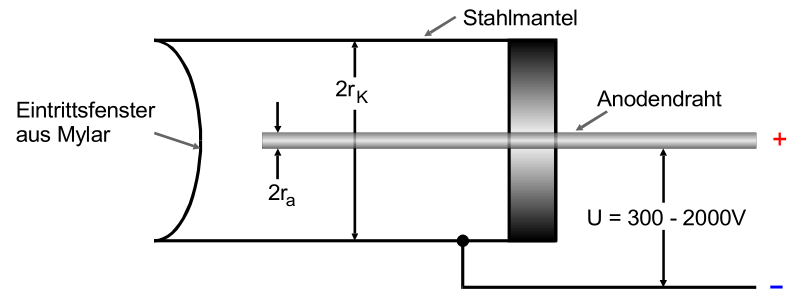
\includegraphics[width=0.7\textwidth]{data/zaehlrohr.png}
    \caption{Schematische Darstellung eines Geiger-Müller-Zählrohres.}
    \label{fig:schemGeiger}
\end{figure}

Die im Zählrohr ablaufenden Vorgänge sind stark abhängig von der im Zylindermantel angelegten Spannung.
Eine Darstellung der emittierten Elektronen ist in \autoref{fig:verlauf} gegenüber der angelegten Spannung in einem Proportionalzählrohr abgebildet.
Es werden fünf verschiedene Teilbereiche unterschieden, die im folgenden näher erläutert werden sollen.
\begin{figure}[H]
    \centering
    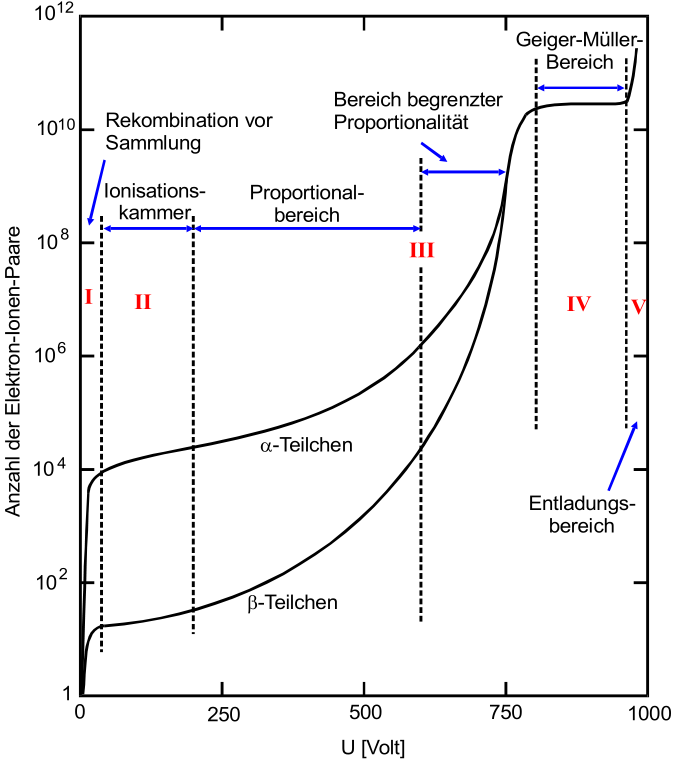
\includegraphics[width=0.5\textwidth]{data/verlauf.png}
    \caption{Anzahl der erzeugten Elektronen in Abhängigkeit der angelegten Spannung $U$.}
    \label{fig:verlauf}
\end{figure}

\begin{enumerate} %Besser nicht in eine Auflistung schreiben, sondern einfach in ABschnitten. Ertsmal ist aber übersichtlicher.
    \item Der erste Teilbereich ist der Bereich, in dem nur ein Teil der erzeugten Elektronen den Draht erreicht, da eine zu kleine Spannung $U$ angelegt ist 
    und der Rest durch Rekombination verloren geht.
    \item Wird eine höhere Spannung $U$ angelegt, so sinkt die Rekombinationswahrscheinlichkeit. Es erreichen deshalb fast alle Elektronen den Anodendraht. 
    Der kontinuierlich fließende Ionisationsstrom ist in diesem Bereich proportional zur Energie und zu der Intensität der einfallenden Strahlung. Ein Gerät,
    das unter ebendiesen Bedingungen arbeitet, stellt eine Vorstufe zu einem Zählrohr dar und wird Ionisationskammer genannt. Weil die Ionisationsströme nur sehr gering sind, kann so ein Gerät nur bei
    hohen Strahlungsintensitäten eingesetzt werden.
    \item Wird die Feldstärke weiter erhöht, so erreicht sie in Drahtnähe so hohe Werte, dass die emittierten Elektronen zwischen den Zusammenstößen mit den Argon-Atomen so viel Energie besitzen, um selber Ionisation zu erzeugen.
    Dieser Vorgang wird Stoßionisation genannt. Durch die von den Elektronen hervorgerufene Ionisation werden weitere Elektronen emittiert und es kommt zu einem lawinenartigen Anstieg ihrer Anzahl, was als Townsend-Lawine beizeichnet wird. 
    Die pro einfallendes Teilchen am Zählrohrdraht gesammelte Ladung $Q$ ist in diesem Teilbereich so groß, dass sie als Ladungsimpuls gemessen werden kann. Dieser Ladungsimpuls kann, aufgrund der weiterhin vorliegenden Proportionalität zwischen Ladung und Energie,
    als Maß für die Teilchenenergie genommen werden. Es ist in diesem Strahlungsbereich also möglich neben der Strahlungsintensität auch die Teilchenenergie zu messen. Aufgrund der erwähnten Proportionalität werden Geräte, die in diesem Teilbereich arbeiten als Proportionalzählrohre bezeichnet.
\end{enumerate}
